% Options for packages loaded elsewhere
\PassOptionsToPackage{unicode}{hyperref}
\PassOptionsToPackage{hyphens}{url}
%
\documentclass[
]{article}
\usepackage{amsmath,amssymb}
\usepackage{iftex}
\ifPDFTeX
  \usepackage[T1]{fontenc}
  \usepackage[utf8]{inputenc}
  \usepackage{textcomp} % provide euro and other symbols
\else % if luatex or xetex
  \usepackage{unicode-math} % this also loads fontspec
  \defaultfontfeatures{Scale=MatchLowercase}
  \defaultfontfeatures[\rmfamily]{Ligatures=TeX,Scale=1}
\fi
\usepackage{lmodern}
\ifPDFTeX\else
  % xetex/luatex font selection
\fi
% Use upquote if available, for straight quotes in verbatim environments
\IfFileExists{upquote.sty}{\usepackage{upquote}}{}
\IfFileExists{microtype.sty}{% use microtype if available
  \usepackage[]{microtype}
  \UseMicrotypeSet[protrusion]{basicmath} % disable protrusion for tt fonts
}{}
\makeatletter
\@ifundefined{KOMAClassName}{% if non-KOMA class
  \IfFileExists{parskip.sty}{%
    \usepackage{parskip}
  }{% else
    \setlength{\parindent}{0pt}
    \setlength{\parskip}{6pt plus 2pt minus 1pt}}
}{% if KOMA class
  \KOMAoptions{parskip=half}}
\makeatother
\usepackage{xcolor}
\usepackage[margin=1in]{geometry}
\usepackage{graphicx}
\makeatletter
\def\maxwidth{\ifdim\Gin@nat@width>\linewidth\linewidth\else\Gin@nat@width\fi}
\def\maxheight{\ifdim\Gin@nat@height>\textheight\textheight\else\Gin@nat@height\fi}
\makeatother
% Scale images if necessary, so that they will not overflow the page
% margins by default, and it is still possible to overwrite the defaults
% using explicit options in \includegraphics[width, height, ...]{}
\setkeys{Gin}{width=\maxwidth,height=\maxheight,keepaspectratio}
% Set default figure placement to htbp
\makeatletter
\def\fps@figure{htbp}
\makeatother
\setlength{\emergencystretch}{3em} % prevent overfull lines
\providecommand{\tightlist}{%
  \setlength{\itemsep}{0pt}\setlength{\parskip}{0pt}}
\setcounter{secnumdepth}{-\maxdimen} % remove section numbering
\ifLuaTeX
  \usepackage{selnolig}  % disable illegal ligatures
\fi
\IfFileExists{bookmark.sty}{\usepackage{bookmark}}{\usepackage{hyperref}}
\IfFileExists{xurl.sty}{\usepackage{xurl}}{} % add URL line breaks if available
\urlstyle{same}
\hypersetup{
  pdftitle={Chapter 1: ADK Community Rarity},
  pdfauthor={Montana},
  hidelinks,
  pdfcreator={LaTeX via pandoc}}

\title{Chapter 1: ADK Community Rarity}
\author{Montana}
\date{2024-02-20}

\begin{document}
\maketitle

\hypertarget{isotopic-perspectives-on-common-and-rare-lake-fishes-trophic-position-niche-overlap-and-niche-size}{%
\section{Isotopic Perspectives on Common and Rare Lake Fishes: Trophic
Position, Niche Overlap, and Niche
Size}\label{isotopic-perspectives-on-common-and-rare-lake-fishes-trophic-position-niche-overlap-and-niche-size}}

\hypertarget{here-is-the-clean-script-for-the-adk-community-species-rarity-manuscript.}{%
\subsection{Here is the clean script for the ADK community + species
rarity
manuscript.}\label{here-is-the-clean-script-for-the-adk-community-species-rarity-manuscript.}}

\begin{verbatim}
##      iso1 iso2 group community
## 1  -28.68 8.50     6         1
## 2  -29.21 8.93     6         1
## 3  -27.88 8.39     6         1
## 4  -29.01 8.54     6         1
## 5  -29.75 7.57    15         1
## 6  -29.66 7.76    15         1
## 7  -29.81 8.10    15         1
## 8  -30.02 7.54    15         1
## 9  -29.80 7.65    15         1
## 10 -30.20 6.88     6         1
## 11 -28.58 6.48     6         1
## 12 -29.14 6.86     6         1
## 13 -30.64 6.84    15         1
## Compiling model graph
##    Resolving undeclared variables
##    Allocating nodes
## Graph information:
##    Observed stochastic nodes: 7
##    Unobserved stochastic nodes: 3
##    Total graph size: 22
## 
## Initializing model
## 
## Compiling model graph
##    Resolving undeclared variables
##    Allocating nodes
## Graph information:
##    Observed stochastic nodes: 6
##    Unobserved stochastic nodes: 3
##    Total graph size: 21
## 
## Initializing model
## 
##      iso1 iso2 group community
## 1  -28.15 7.89     6         2
## 2  -29.52 7.92    19         2
## 3  -30.00 7.16    15         2
## 4  -30.37 7.54    15         2
## 5  -31.84 8.29    19         2
## 6  -28.92 7.17     6         2
## 7  -30.40 7.36    19         2
## 8  -28.81 6.79    15         2
## 9  -28.72 6.50     6         2
## 10 -29.70 7.58     6         2
## 11 -29.43 8.01     6         2
## 12 -30.92 7.33    15         2
## 13 -28.80 7.11     6         2
## 14 -30.56 7.18    15         2
## 15 -30.99 8.36    19         2
## 16 -29.93 7.31    15         2
## 17 -31.65 7.75    19         2
## Compiling model graph
##    Resolving undeclared variables
##    Allocating nodes
## Graph information:
##    Observed stochastic nodes: 6
##    Unobserved stochastic nodes: 3
##    Total graph size: 21
## 
## Initializing model
## 
## Compiling model graph
##    Resolving undeclared variables
##    Allocating nodes
## Graph information:
##    Observed stochastic nodes: 5
##    Unobserved stochastic nodes: 3
##    Total graph size: 20
## 
## Initializing model
## 
## Compiling model graph
##    Resolving undeclared variables
##    Allocating nodes
## Graph information:
##    Observed stochastic nodes: 6
##    Unobserved stochastic nodes: 3
##    Total graph size: 21
## 
## Initializing model
## 
##      iso1  iso2 group community
## 1  -33.08  9.41    14         3
## 2  -33.49  9.56    19         3
## 3  -32.10  7.51    18         3
## 4  -31.44  8.64     6         3
## 5  -29.56  9.04     6         3
## 6  -33.99  8.09    18         3
## 7  -33.17  9.46    19         3
## 8  -32.64  8.19    18         3
## 9  -28.16  8.46     6         3
## 10 -31.14  8.96     6         3
## 11 -32.52  9.24     6         3
## 12 -30.10  8.94     6         3
## 13 -32.41  8.73    19         3
## 14 -32.84  7.57    18         3
## 15 -33.36  8.97    19         3
## 16 -34.08  8.05    18         3
## 17 -34.38  9.17    18         3
## 18 -32.66  8.57    18         3
## 19 -33.22  9.19    19         3
## 20 -32.91  7.67    18         3
## 21 -32.06  9.12    14         3
## 22 -33.63  9.75    14         3
## 23 -33.30  9.54    14         3
## 24 -33.12  9.51    14         3
## 25 -35.53 10.05    14         3
## 26 -34.16  9.21    14         3
## 27 -32.02  9.24    14         3
## 28 -31.38  8.94    14         3
## 29 -32.29  8.92    14         3
## 30 -33.41  9.68    14         3
## Compiling model graph
##    Resolving undeclared variables
##    Allocating nodes
## Graph information:
##    Observed stochastic nodes: 11
##    Unobserved stochastic nodes: 3
##    Total graph size: 26
## 
## Initializing model
## 
## Compiling model graph
##    Resolving undeclared variables
##    Allocating nodes
## Graph information:
##    Observed stochastic nodes: 5
##    Unobserved stochastic nodes: 3
##    Total graph size: 20
## 
## Initializing model
## 
## Compiling model graph
##    Resolving undeclared variables
##    Allocating nodes
## Graph information:
##    Observed stochastic nodes: 8
##    Unobserved stochastic nodes: 3
##    Total graph size: 23
## 
## Initializing model
## 
## Compiling model graph
##    Resolving undeclared variables
##    Allocating nodes
## Graph information:
##    Observed stochastic nodes: 6
##    Unobserved stochastic nodes: 3
##    Total graph size: 21
## 
## Initializing model
## 
##     iso1 iso2 group community
## 1 -29.56 8.06     6         4
## 2 -31.25 9.40     6         4
## 3 -30.34 8.98     6         4
## 4 -29.31 8.32     6         4
## 5 -30.19 8.60     6         4
## Compiling model graph
##    Resolving undeclared variables
##    Allocating nodes
## Graph information:
##    Observed stochastic nodes: 5
##    Unobserved stochastic nodes: 3
##    Total graph size: 20
## 
## Initializing model
## 
##      iso1 iso2 group community
## 1  -29.38 7.72    15         5
## 2  -29.47 7.23    15         5
## 3  -30.64 6.99    18         5
## 4  -29.05 7.85    15         5
## 5  -29.31 7.40    15         5
## 6  -30.53 6.88    18         5
## 7  -28.73 7.50    15         5
## 8  -28.53 7.10    13         5
## 9  -31.45 6.72    13         5
## 10 -31.30 7.12    13         5
## 11 -31.03 7.05    13         5
## 12 -29.20 7.43    18         5
## 13 -28.30 7.24    13         5
## 14 -32.23 6.74    13         5
## 15 -30.22 7.31    15         5
## 16 -30.83 7.22    15         5
## 17 -30.44 7.51    15         5
## 18 -29.99 6.77    15         5
## 19 -30.41 7.65    15         5
## 20 -29.56 7.80    15         5
## 21 -29.98 8.02    18         5
## 22 -30.99 7.27    15         5
## Compiling model graph
##    Resolving undeclared variables
##    Allocating nodes
## Graph information:
##    Observed stochastic nodes: 12
##    Unobserved stochastic nodes: 3
##    Total graph size: 27
## 
## Initializing model
## 
## Compiling model graph
##    Resolving undeclared variables
##    Allocating nodes
## Graph information:
##    Observed stochastic nodes: 4
##    Unobserved stochastic nodes: 3
##    Total graph size: 19
## 
## Initializing model
## 
## Compiling model graph
##    Resolving undeclared variables
##    Allocating nodes
## Graph information:
##    Observed stochastic nodes: 6
##    Unobserved stochastic nodes: 3
##    Total graph size: 21
## 
## Initializing model
## 
##      iso1 iso2 group community
## 1  -30.03 6.96    20         7
## 2  -28.06 6.92     1         7
## 3  -26.34 6.19     9         7
## 4  -26.36 5.94     9         7
## 5  -26.35 4.77     9         7
## 6  -26.16 6.68     9         7
## 7  -27.15 6.48     9         7
## 8  -24.91 9.10     9         7
## 9  -25.54 6.22     6         7
## 10 -25.22 6.77     6         7
## 11 -25.65 8.10     6         7
## 12 -25.72 6.38     6         7
## 13 -27.14 6.51     4         7
## 14 -27.48 5.84     4         7
## 15 -26.95 6.03     4         7
## 16 -24.03 6.08     4         7
## 17 -26.40 6.20     4         7
## 18 -27.62 5.98     4         7
## 19 -27.17 6.72     4         7
## 20 -24.26 6.31     4         7
## 21 -27.02 5.89     4         7
## 22 -28.33 8.38     1         7
## 23 -27.28 8.12    20         7
## 24 -27.30 7.61    20         7
## 25 -28.85 6.94    20         7
## 26 -30.02 6.15     1         7
## 27 -26.69 6.10     9         7
## 28 -25.71 6.31     9         7
## 29 -26.53 6.31     9         7
## 30 -26.07 7.41     6         7
## 31 -26.41 6.67     6         7
## 32 -25.14 7.79     6         7
## 33 -26.45 6.60     4         7
## 34 -25.78 5.98     9         7
## 35 -24.54 8.03     6         7
## 36 -26.36 6.64     6         7
## 37 -24.77 6.41     6         7
## 38 -26.50 7.50     6         7
## 39 -27.13 5.92     4         7
## 40 -26.81 5.55     4         7
## 41 -26.25 5.26     4         7
## 42 -27.76 8.55     1         7
## 43 -27.31 7.37     1         7
## 44 -29.16 6.36     1         7
## 45 -27.15 6.54     9         7
## 46 -28.20 6.69     9         7
## 47 -27.28 5.92     9         7
## 48 -27.20 6.53     9         7
## 49 -27.34 6.53     9         7
## 50 -28.71 5.17     9         7
## 51 -27.41 5.80     9         7
## 52 -26.74 7.05     9         7
## 53 -27.29 6.74     9         7
## 54 -27.44 6.39     9         7
## 55 -27.68 5.64     9         7
## 56 -29.16 5.69     9         7
## 57 -29.36 4.94     4         7
## 58 -29.52 5.55     4         7
## 59 -28.78 5.41     4         7
## 60 -27.39 6.05    19         7
## 61 -26.79 5.93    19         7
## 62 -28.94 7.45    15         7
## 63 -29.32 7.39    15         7
## 64 -27.86 7.03    15         7
## 65 -28.71 7.07    15         7
## 66 -29.04 7.34    15         7
## 67 -28.88 6.95    15         7
## 68 -31.32 7.10    15         7
## 69 -29.15 6.27     9         7
## 70 -28.25 6.40    15         7
## 71 -29.61 7.37     1         7
## 72 -26.49 5.72    20         7
## 73 -34.58 5.36    20         7
## 74 -33.91 5.43    20         7
## 75 -32.24 5.97    20         7
## 76 -26.04 5.65    20         7
## 77 -28.40 6.84    15         7
## 78 -26.94 6.64    19         7
## 79 -28.30 6.79    15         7
## 80 -26.66 6.28    19         7
## 81 -28.29 6.30    19         7
## 82 -28.39 7.17    15         7
## 83 -27.65 6.22    19         7
## 84 -26.36 6.19    19         7
## 85 -28.55 5.23     4         7
## 86 -26.30 5.56    20         7
## 87 -26.80 7.33    20         7
## 88 -27.35 5.95     9         7
## 89 -28.61 7.09    15         7
## 90 -27.34 5.67    20         7
## 91 -26.94 5.38     4         7
## 92 -23.26 9.18     9         7
## 93 -26.21 5.14    19         7
## 94 -26.28 6.28    19         7
## Compiling model graph
##    Resolving undeclared variables
##    Allocating nodes
## Graph information:
##    Observed stochastic nodes: 12
##    Unobserved stochastic nodes: 3
##    Total graph size: 27
## 
## Initializing model
## 
## Compiling model graph
##    Resolving undeclared variables
##    Allocating nodes
## Graph information:
##    Observed stochastic nodes: 7
##    Unobserved stochastic nodes: 3
##    Total graph size: 22
## 
## Initializing model
## 
## Compiling model graph
##    Resolving undeclared variables
##    Allocating nodes
## Graph information:
##    Observed stochastic nodes: 25
##    Unobserved stochastic nodes: 3
##    Total graph size: 40
## 
## Initializing model
## 
## Compiling model graph
##    Resolving undeclared variables
##    Allocating nodes
## Graph information:
##    Observed stochastic nodes: 11
##    Unobserved stochastic nodes: 3
##    Total graph size: 26
## 
## Initializing model
## 
## Compiling model graph
##    Resolving undeclared variables
##    Allocating nodes
## Graph information:
##    Observed stochastic nodes: 18
##    Unobserved stochastic nodes: 3
##    Total graph size: 33
## 
## Initializing model
## 
## Compiling model graph
##    Resolving undeclared variables
##    Allocating nodes
## Graph information:
##    Observed stochastic nodes: 9
##    Unobserved stochastic nodes: 3
##    Total graph size: 24
## 
## Initializing model
## 
## Compiling model graph
##    Resolving undeclared variables
##    Allocating nodes
## Graph information:
##    Observed stochastic nodes: 12
##    Unobserved stochastic nodes: 3
##    Total graph size: 27
## 
## Initializing model
## 
##      iso1  iso2 group community
## 1  -27.15  7.78     3         8
## 2  -29.46  7.61     3         8
## 3  -24.99  7.59     3         8
## 4  -22.84  8.92     6         8
## 5  -25.38  8.12     3         8
## 6  -24.92  7.80     3         8
## 7  -23.59  8.11     6         8
## 8  -23.95  9.75     6         8
## 9  -25.45  8.16    24         8
## 10 -29.79  9.15    22         8
## 11 -25.88  7.89    24         8
## 12 -25.30  7.41     3         8
## 13 -26.66  7.67     3         8
## 14 -26.07  7.96     3         8
## 15 -23.54  7.78     3         8
## 16 -24.82  7.57     3         8
## 17 -29.70  9.38    22         8
## 18 -27.58  8.64    24         8
## 19 -28.27  9.48    24         8
## 20 -29.12  8.43    22         8
## 21 -25.78  8.24     3         8
## 22 -25.73  7.22     3         8
## 23 -26.79  7.45     3         8
## 24 -25.52  6.14     6         8
## 25 -23.48  8.15     6         8
## 26 -28.66  7.62     3         8
## 27 -25.93  9.42    24         8
## 28 -30.22  9.01    22         8
## 29 -23.39  8.02     6         8
## 30 -28.50  8.81     3         8
## 31 -22.25  7.72     3         8
## 32 -26.13  7.59     3         8
## 33 -24.53  8.85     6         8
## 34 -24.87  7.60     3         8
## 35 -22.94  8.32     3         8
## 36 -26.51  7.17    22         8
## 37 -25.20  7.94     3         8
## 38 -24.83  8.47     6         8
## 39 -23.03  8.18     6         8
## 40 -27.73  7.22     3         8
## 41 -24.84  8.76     3         8
## 42 -27.04  9.05     3         8
## 43 -23.12  9.32     6         8
## 44 -22.17  8.59     6         8
## 45 -25.27 10.80    24         8
## 46 -26.82  6.50     6         8
## 47 -27.61  7.74     3         8
## 48 -26.65  8.33    24         8
## 49 -26.20  8.62     3         8
## 50 -20.85  8.58     3         8
## 51 -25.90  7.56     3         8
## 52 -26.69  7.70     3         8
## Compiling model graph
##    Resolving undeclared variables
##    Allocating nodes
## Graph information:
##    Observed stochastic nodes: 28
##    Unobserved stochastic nodes: 3
##    Total graph size: 43
## 
## Initializing model
## 
## Compiling model graph
##    Resolving undeclared variables
##    Allocating nodes
## Graph information:
##    Observed stochastic nodes: 12
##    Unobserved stochastic nodes: 3
##    Total graph size: 27
## 
## Initializing model
## 
## Compiling model graph
##    Resolving undeclared variables
##    Allocating nodes
## Graph information:
##    Observed stochastic nodes: 7
##    Unobserved stochastic nodes: 3
##    Total graph size: 22
## 
## Initializing model
## 
## Compiling model graph
##    Resolving undeclared variables
##    Allocating nodes
## Graph information:
##    Observed stochastic nodes: 5
##    Unobserved stochastic nodes: 3
##    Total graph size: 20
## 
## Initializing model
## 
##      iso1 iso2 group community
## 1  -29.48 7.28     1         9
## 2  -28.47 5.58    19         9
## 3  -29.87 6.24    19         9
## 4  -27.67 6.24    19         9
## 5  -28.03 6.85    19         9
## 6  -28.81 7.08    19         9
## 7  -30.88 6.37    19         9
## 8  -29.50 6.46    19         9
## 9  -28.81 7.38    19         9
## 10 -34.17 8.09    19         9
## 11 -29.71 6.57    19         9
## 12 -29.63 7.40    19         9
## 13 -29.62 7.39    19         9
## 14 -30.05 6.80    19         9
## 15 -29.28 6.78    19         9
## 16 -29.04 6.44    19         9
## 17 -30.03 7.34    19         9
## 18 -30.58 7.98    15         9
## 19 -30.32 7.14    15         9
## 20 -26.79 7.01     6         9
## 21 -28.45 7.26    15         9
## 22 -29.78 7.16    15         9
## 23 -27.47 6.25     6         9
## 24 -27.74 6.03    19         9
## 25 -27.97 7.14    19         9
## 26 -29.31 7.47     1         9
## 27 -28.82 7.15     1         9
## 28 -30.77 6.79     1         9
## 29 -29.25 7.30    15         9
## 30 -28.64 6.73    15         9
## 31 -31.63 7.04    15         9
## 32 -32.06 6.77    15         9
## 33 -31.93 7.73    15         9
## 34 -31.56 7.70    15         9
## 35 -29.78 7.16    15         9
## 36 -31.75 8.08    15         9
## 37 -31.08 7.77    15         9
## 38 -30.12 4.47    15         9
## 39 -31.37 5.68    25         9
## 40 -30.04 7.05    19         9
## 41 -29.63 7.91    15         9
## 42 -28.20 7.21    19         9
## 43 -31.51 7.46    15         9
## 44 -30.41 7.60    15         9
## 45 -30.74 5.11    25         9
## 46 -30.94 5.80     1         9
## 47 -31.23 7.21    15         9
## 48 -30.90 5.48    25         9
## 49 -30.14 7.20    15         9
## 50 -28.24 6.84    19         9
## 51 -28.36 7.22    15         9
## 52 -28.50 7.43    19         9
## 53 -31.12 7.84    15         9
## 54 -31.26 7.57    15         9
## 55 -29.59 6.21    19         9
## 56 -29.54 4.79    25         9
## 57 -28.96 6.62     6         9
## 58 -30.42 4.61    25         9
## 59 -28.52 7.67     1         9
## 60 -29.17 7.56     1         9
## 61 -28.09 7.69     6         9
## 62 -26.96 6.59     6         9
## 63 -26.81 7.41     6         9
## Compiling model graph
##    Resolving undeclared variables
##    Allocating nodes
## Graph information:
##    Observed stochastic nodes: 7
##    Unobserved stochastic nodes: 3
##    Total graph size: 22
## 
## Initializing model
## 
## Compiling model graph
##    Resolving undeclared variables
##    Allocating nodes
## Graph information:
##    Observed stochastic nodes: 23
##    Unobserved stochastic nodes: 3
##    Total graph size: 38
## 
## Initializing model
## 
## Compiling model graph
##    Resolving undeclared variables
##    Allocating nodes
## Graph information:
##    Observed stochastic nodes: 22
##    Unobserved stochastic nodes: 3
##    Total graph size: 37
## 
## Initializing model
## 
## Compiling model graph
##    Resolving undeclared variables
##    Allocating nodes
## Graph information:
##    Observed stochastic nodes: 6
##    Unobserved stochastic nodes: 3
##    Total graph size: 21
## 
## Initializing model
## 
## Compiling model graph
##    Resolving undeclared variables
##    Allocating nodes
## Graph information:
##    Observed stochastic nodes: 5
##    Unobserved stochastic nodes: 3
##    Total graph size: 20
## 
## Initializing model
## 
##     iso1 iso2 group community
## 1 -30.12 8.39     6        10
## 2 -27.92 7.44     6        10
## 3 -27.39 8.14     6        10
## 4 -27.35 8.54     6        10
## 5 -28.06 7.63     6        10
## 6 -28.86 7.95     6        10
## Compiling model graph
##    Resolving undeclared variables
##    Allocating nodes
## Graph information:
##    Observed stochastic nodes: 6
##    Unobserved stochastic nodes: 3
##    Total graph size: 21
## 
## Initializing model
## 
##      iso1 iso2 group community
## 1  -29.60 7.49    19        11
## 2  -28.95 7.52    19        11
## 3  -29.45 7.68    19        11
## 4  -29.16 8.19     6        11
## 5  -28.51 7.93     6        11
## 6  -29.34 7.71    19        11
## 7  -28.46 7.78    19        11
## 8  -30.03 6.82    19        11
## 9  -29.23 7.62    19        11
## 10 -30.17 7.97    19        11
## 11 -29.97 7.07    19        11
## 12 -28.91 6.63     6        11
## 13 -27.09 7.97     6        11
## 14 -28.50 8.41     6        11
## 15 -28.58 8.66     6        11
## 16 -29.02 7.53    19        11
## Compiling model graph
##    Resolving undeclared variables
##    Allocating nodes
## Graph information:
##    Observed stochastic nodes: 10
##    Unobserved stochastic nodes: 3
##    Total graph size: 25
## 
## Initializing model
## 
## Compiling model graph
##    Resolving undeclared variables
##    Allocating nodes
## Graph information:
##    Observed stochastic nodes: 6
##    Unobserved stochastic nodes: 3
##    Total graph size: 21
## 
## Initializing model
## 
##      iso1 iso2 group community
## 1  -26.19 8.17    22        12
## 2  -26.97 7.93    22        12
## 3  -27.03 7.99    22        12
## 4  -25.78 8.47    22        12
## 5  -26.33 8.65    22        12
## 6  -26.62 7.92    22        12
## 7  -26.67 8.38    22        12
## 8  -27.21 7.99    22        12
## 9  -25.95 8.51    22        12
## 10 -25.64 8.61    22        12
## 11 -25.55 9.01    22        12
## 12 -26.30 8.85    22        12
## Compiling model graph
##    Resolving undeclared variables
##    Allocating nodes
## Graph information:
##    Observed stochastic nodes: 12
##    Unobserved stochastic nodes: 3
##    Total graph size: 27
## 
## Initializing model
## 
##      iso1 iso2 group community
## 1  -27.43 7.75     6        13
## 2  -27.47 8.19     6        13
## 3  -27.52 7.97     6        13
## 4  -28.95 8.37     6        13
## 5  -27.06 7.73     6        13
## 6  -26.95 7.88     6        13
## 7  -27.92 8.35     6        13
## 8  -29.94 7.55     6        13
## 9  -27.70 8.12     6        13
## 10 -30.08 7.60     6        13
## 11 -28.76 8.60     6        13
## 12 -28.39 8.67     6        13
## 13 -28.26 8.21     6        13
## 14 -28.68 8.04     6        13
## 15 -28.00 7.94     6        13
## Compiling model graph
##    Resolving undeclared variables
##    Allocating nodes
## Graph information:
##    Observed stochastic nodes: 15
##    Unobserved stochastic nodes: 3
##    Total graph size: 30
## 
## Initializing model
## 
##      iso1 iso2 group community
## 1  -30.49 8.24     6        14
## 2  -30.01 9.02     6        14
## 3  -30.22 8.09     6        14
## 4  -30.87 9.09     6        14
## 5  -31.15 8.62     6        14
## 6  -30.58 8.50     6        14
## 7  -31.17 8.81     6        14
## 8  -30.46 9.22     6        14
## 9  -30.51 8.71     6        14
## 10 -31.75 9.53     6        14
## 11 -32.71 9.58    19        14
## 12 -31.11 8.58    19        14
## 13 -31.03 9.55    19        14
## 14 -30.76 7.49    19        14
## 15 -31.07 9.34    19        14
## 16 -30.30 8.48    19        14
## 17 -32.51 7.80    19        14
## 18 -31.28 9.55    19        14
## 19 -31.55 9.98    19        14
## 20 -30.90 7.82    19        14
## 21 -32.24 8.71    19        14
## 22 -30.80 7.26    19        14
## 23 -32.47 8.93    19        14
## 24 -31.35 8.03     6        14
## Compiling model graph
##    Resolving undeclared variables
##    Allocating nodes
## Graph information:
##    Observed stochastic nodes: 11
##    Unobserved stochastic nodes: 3
##    Total graph size: 26
## 
## Initializing model
## 
## Compiling model graph
##    Resolving undeclared variables
##    Allocating nodes
## Graph information:
##    Observed stochastic nodes: 13
##    Unobserved stochastic nodes: 3
##    Total graph size: 28
## 
## Initializing model
## 
##      iso1  iso2 group community
## 1  -34.40  7.86    18        15
## 2  -35.06  8.61    18        15
## 3  -34.22  7.80    18        15
## 4  -33.80  8.83    14        15
## 5  -35.69  9.17    18        15
## 6  -32.72  7.99    18        15
## 7  -34.25  8.50    18        15
## 8  -33.21  7.31    18        15
## 9  -28.01  8.00    19        15
## 10 -33.25  8.71    19        15
## 11 -33.73  7.84    18        15
## 12 -35.81  9.22    18        15
## 13 -32.14  8.95    19        15
## 14 -33.83  8.70    18        15
## 15 -32.74  8.94    19        15
## 16 -33.70  9.04    14        15
## 17 -34.98  9.61    19        15
## 18 -34.76  8.54    18        15
## 19 -34.11  7.94    18        15
## 20 -33.97  7.80    18        15
## 21 -33.38  8.40    19        15
## 22 -34.26  9.35    19        15
## 23 -29.46  8.32    19        15
## 24 -33.40  7.55    18        15
## 25 -33.07  8.14    18        15
## 26 -34.99  9.47    19        15
## 27 -31.01  7.59    19        15
## 28 -35.00  8.59    18        15
## 29 -29.81  7.92     6        15
## 30 -32.04  8.64     6        15
## 31 -33.48  9.13    19        15
## 32 -32.92  9.44    14        15
## 33 -31.71  8.74     6        15
## 34 -31.12  8.32     6        15
## 35 -31.28  9.48     6        15
## 36 -32.43  8.57    19        15
## 37 -34.52 10.11    19        15
## 38 -30.44  8.12     6        15
## 39 -34.75  8.11    18        15
## 40 -32.52  7.52    18        15
## 41 -29.98  8.54     6        15
## 42 -34.23  9.57    19        15
## 43 -32.60  9.22     6        15
## 44 -33.45  9.56    19        15
## 45 -33.70  8.97    19        15
## 46 -32.80  9.63    19        15
## 47 -33.57  9.80    14        15
## 48 -34.60  9.31    14        15
## 49 -32.76  8.53     6        15
## 50 -32.25  8.17     6        15
## 51 -32.20  7.07    18        15
## 52 -33.33  7.86    18        15
## 53 -32.04  8.24    14        15
## 54 -33.72  9.11    14        15
## 55 -29.01  8.98     6        15
## 56 -33.40  9.45    14        15
## Compiling model graph
##    Resolving undeclared variables
##    Allocating nodes
## Graph information:
##    Observed stochastic nodes: 20
##    Unobserved stochastic nodes: 3
##    Total graph size: 35
## 
## Initializing model
## 
## Compiling model graph
##    Resolving undeclared variables
##    Allocating nodes
## Graph information:
##    Observed stochastic nodes: 8
##    Unobserved stochastic nodes: 3
##    Total graph size: 23
## 
## Initializing model
## 
## Compiling model graph
##    Resolving undeclared variables
##    Allocating nodes
## Graph information:
##    Observed stochastic nodes: 17
##    Unobserved stochastic nodes: 3
##    Total graph size: 32
## 
## Initializing model
## 
## Compiling model graph
##    Resolving undeclared variables
##    Allocating nodes
## Graph information:
##    Observed stochastic nodes: 11
##    Unobserved stochastic nodes: 3
##    Total graph size: 26
## 
## Initializing model
## 
##      iso1 iso2 group community
## 1  -30.54 5.72     1        16
## 2  -30.42 6.29     1        16
## 3  -32.02 6.81     1        16
## 4  -28.68 7.68     6        16
## 5  -30.56 7.12     6        16
## 6  -31.34 9.20     6        16
## 7  -28.09 6.44     6        16
## 8  -31.15 6.58     1        16
## 9  -30.12 6.68     1        16
## 10 -31.92 6.30     1        16
## 11 -31.45 9.04     6        16
## 12 -32.27 8.23     6        16
## 13 -28.66 7.61     6        16
## 14 -30.81 7.45     6        16
## 15 -31.77 9.16     6        16
## Compiling model graph
##    Resolving undeclared variables
##    Allocating nodes
## Graph information:
##    Observed stochastic nodes: 6
##    Unobserved stochastic nodes: 3
##    Total graph size: 21
## 
## Initializing model
## 
## Compiling model graph
##    Resolving undeclared variables
##    Allocating nodes
## Graph information:
##    Observed stochastic nodes: 9
##    Unobserved stochastic nodes: 3
##    Total graph size: 24
## 
## Initializing model
## 
##      iso1 iso2 group community
## 1  -24.50 6.41     9        17
## 2  -20.17 6.29    20        17
## 3  -21.65 6.94    20        17
## 4  -20.52 6.83    20        17
## 5  -30.26 5.27    20        17
## 6  -22.24 6.32    20        17
## 7  -20.25 7.39    20        17
## 8  -22.79 6.41    20        17
## 9  -25.07 6.42    20        17
## 10 -20.04 5.07    25        17
## 11 -27.27 5.89    17        17
## 12 -25.17 6.32    17        17
## 13 -21.54 4.90    25        17
## 14 -23.82 5.71    20        17
## 15 -26.87 5.80    17        17
## 16 -26.63 6.55    17        17
## 17 -23.64 6.26     6        17
## 18 -25.73 6.00     6        17
## 19 -24.31 6.52     6        17
## 20 -24.67 6.52     9        17
## 21 -25.28 6.14     9        17
## 22 -27.19 7.31     9        17
## 23 -24.28 5.63     9        17
## 24 -24.90 6.30     9        17
## 25 -24.31 5.68     9        17
## 26 -24.15 5.98     9        17
## 27 -24.86 5.58     9        17
## 28 -25.68 6.00     9        17
## 29 -25.48 6.17     9        17
## 30 -24.27 6.50     9        17
## 31 -23.14 5.90     9        17
## 32 -23.84 6.44     9        17
## 33 -24.64 5.61     9        17
## 34 -24.51 5.84     9        17
## 35 -23.84 7.06    20        17
## 36 -25.66 7.01    20        17
## 37 -24.81 6.53    20        17
## 38 -18.83 6.10    20        17
## 39 -23.31 5.83    20        17
## 40 -21.20 6.43    20        17
## 41 -22.81 5.74    20        17
## 42 -25.16 5.71    20        17
## 43 -26.99 6.24     6        17
## 44 -22.01 6.12     6        17
## 45 -24.24 5.17    17        17
## 46 -23.79 5.45    17        17
## 47 -22.34 5.66    17        17
## 48 -24.93 5.46    17        17
## 49 -23.14 5.63    17        17
## 50 -21.95 5.88    17        17
## 51 -21.73 5.19    17        17
## 52 -20.82 6.33    17        17
## 53 -22.04 5.73    25        17
## 54 -21.55 5.44    25        17
## 55 -26.78 4.61    25        17
## 56 -24.68 6.18     9        17
## 57 -26.01 5.81     9        17
## 58 -24.13 5.46     9        17
## 59 -25.20 6.76     9        17
## 60 -23.93 5.83     9        17
## 61 -24.31 5.61     9        17
## 62 -24.89 5.84     9        17
## 63 -24.81 5.98     9        17
## 64 -20.99 7.88    20        17
## 65 -20.22 6.65    20        17
## 66 -22.40 5.88    20        17
## 67 -19.53 6.56    20        17
## 68 -22.22 6.18    20        17
## 69 -20.37 6.53    20        17
## 70 -24.59 5.86    20        17
## 71 -25.32 7.49    23        17
## 72 -20.11 6.76    23        17
## 73 -24.61 7.33    23        17
## 74 -25.09 6.83    23        17
## 75 -23.89 6.27    23        17
## 76 -24.88 6.41    23        17
## 77 -21.01 6.76    23        17
## 78 -24.90 6.55    23        17
## 79 -23.20 6.10    23        17
## 80 -21.48 6.88    23        17
## 81 -25.29 6.51    23        17
## 82 -25.93 4.99    23        17
## 83 -25.34 6.60    23        17
## 84 -24.05 6.08    23        17
## 85 -25.11 6.72    23        17
## 86 -24.85 7.13    23        17
## 87 -24.81 6.75    23        17
## 88 -24.75 6.62    23        17
## 89 -24.57 7.50    23        17
## 90 -25.34 6.18    23        17
## 91 -25.61 5.71    23        17
## 92 -24.19 6.88    23        17
## Compiling model graph
##    Resolving undeclared variables
##    Allocating nodes
## Graph information:
##    Observed stochastic nodes: 24
##    Unobserved stochastic nodes: 3
##    Total graph size: 39
## 
## Initializing model
## 
## Compiling model graph
##    Resolving undeclared variables
##    Allocating nodes
## Graph information:
##    Observed stochastic nodes: 24
##    Unobserved stochastic nodes: 3
##    Total graph size: 39
## 
## Initializing model
## 
## Compiling model graph
##    Resolving undeclared variables
##    Allocating nodes
## Graph information:
##    Observed stochastic nodes: 5
##    Unobserved stochastic nodes: 3
##    Total graph size: 20
## 
## Initializing model
## 
## Compiling model graph
##    Resolving undeclared variables
##    Allocating nodes
## Graph information:
##    Observed stochastic nodes: 12
##    Unobserved stochastic nodes: 3
##    Total graph size: 27
## 
## Initializing model
## 
## Compiling model graph
##    Resolving undeclared variables
##    Allocating nodes
## Graph information:
##    Observed stochastic nodes: 5
##    Unobserved stochastic nodes: 3
##    Total graph size: 20
## 
## Initializing model
## 
## Compiling model graph
##    Resolving undeclared variables
##    Allocating nodes
## Graph information:
##    Observed stochastic nodes: 22
##    Unobserved stochastic nodes: 3
##    Total graph size: 37
## 
## Initializing model
## 
##      iso1 iso2 group community
## 1  -25.69 6.91     6        19
## 2  -24.89 6.95     6        19
## 3  -25.78 6.48     2        19
## 4  -25.71 5.86     2        19
## 5  -27.17 5.25     6        19
## 6  -27.99 6.22     4        19
## 7  -25.49 6.16     4        19
## 8  -27.07 7.45    20        19
## 9  -30.45 7.47     1        19
## 10 -31.32 7.68    15        19
## 11 -30.35 8.05     1        19
## 12 -30.17 7.95     1        19
## 13 -25.49 6.69     6        19
## 14 -28.14 7.76    20        19
## 15 -25.45 7.37     6        19
## 16 -29.08 7.57    20        19
## 17 -27.88 8.36    20        19
## 18 -25.71 7.07     6        19
## 19 -27.35 6.70     2        19
## 20 -26.14 7.05     6        19
## 21 -26.92 8.16     1        19
## 22 -25.49 6.62     6        19
## 23 -25.40 6.54     1        19
## 24 -27.12 7.47     1        19
## 25 -25.46 5.99     4        19
## 26 -27.27 5.86     4        19
## 27 -26.91 5.49     4        19
## 28 -25.69 4.42     6        19
## 29 -28.17 6.54    15        19
## 30 -24.86 7.51     6        19
## 31 -25.87 6.84     6        19
## 32 -29.36 7.11    15        19
## 33 -26.50 6.69     6        19
## 34 -26.21 6.53     6        19
## 35 -26.72 6.98     6        19
## 36 -26.56 6.44     6        19
## 37 -26.25 6.98     6        19
## 38 -26.63 8.03    15        19
## 39 -30.21 4.43    15        19
## 40 -26.90 6.52     2        19
## 41 -26.40 6.09     2        19
## 42 -26.94 6.45     2        19
## 43 -28.39 7.59    20        19
## 44 -30.89 6.66    20        19
## 45 -25.75 6.74     6        19
## 46 -29.01 6.91    20        19
## 47 -28.13 6.93     1        19
## 48 -27.23 8.08     1        19
## 49 -27.76 6.74     1        19
## 50 -25.35 6.04     2        19
## 51 -25.50 6.93     6        19
## 52 -26.02 6.36     6        19
## 53 -25.90 6.32     4        19
## 54 -27.46 5.70     6        19
## 55 -25.95 6.50     6        19
## 56 -26.51 7.11     4        19
## 57 -25.55 6.26     2        19
## 58 -24.86 6.26     6        19
## 59 -24.89 6.29     4        19
## 60 -28.50 5.49     4        19
## 61 -25.40 5.91     4        19
## 62 -27.20 6.06     4        19
## 63 -30.08 5.35     4        19
## 64 -29.96 5.08     4        19
## 65 -26.31 6.39     2        19
## 66 -26.09 4.79    12        19
## 67 -25.88 4.50    12        19
## 68 -25.33 3.92    12        19
## 69 -27.93 4.48    12        19
## 70 -25.32 4.94    12        19
## 71 -25.48 3.99    12        19
## 72 -24.00 4.14    12        19
## 73 -22.86 4.50    12        19
## 74 -25.58 4.29    12        19
## 75 -27.58 4.31    12        19
## 76 -25.88 4.05    12        19
## 77 -27.23 3.85    12        19
## 78 -26.60 3.06    12        19
## 79 -26.05 6.25    12        19
## 80 -26.23 3.97    12        19
## Compiling model graph
##    Resolving undeclared variables
##    Allocating nodes
## Graph information:
##    Observed stochastic nodes: 22
##    Unobserved stochastic nodes: 3
##    Total graph size: 37
## 
## Initializing model
## 
## Compiling model graph
##    Resolving undeclared variables
##    Allocating nodes
## Graph information:
##    Observed stochastic nodes: 9
##    Unobserved stochastic nodes: 3
##    Total graph size: 24
## 
## Initializing model
## 
## Compiling model graph
##    Resolving undeclared variables
##    Allocating nodes
## Graph information:
##    Observed stochastic nodes: 13
##    Unobserved stochastic nodes: 3
##    Total graph size: 28
## 
## Initializing model
## 
## Compiling model graph
##    Resolving undeclared variables
##    Allocating nodes
## Graph information:
##    Observed stochastic nodes: 7
##    Unobserved stochastic nodes: 3
##    Total graph size: 22
## 
## Initializing model
## 
## Compiling model graph
##    Resolving undeclared variables
##    Allocating nodes
## Graph information:
##    Observed stochastic nodes: 9
##    Unobserved stochastic nodes: 3
##    Total graph size: 24
## 
## Initializing model
## 
## Compiling model graph
##    Resolving undeclared variables
##    Allocating nodes
## Graph information:
##    Observed stochastic nodes: 5
##    Unobserved stochastic nodes: 3
##    Total graph size: 20
## 
## Initializing model
## 
## Compiling model graph
##    Resolving undeclared variables
##    Allocating nodes
## Graph information:
##    Observed stochastic nodes: 15
##    Unobserved stochastic nodes: 3
##    Total graph size: 30
## 
## Initializing model
## 
##     iso1 iso2 group community
## 1 -24.43 7.75     6        20
## 2 -23.85 8.62     6        20
## 3 -24.56 8.63     6        20
## 4 -24.11 8.55     6        20
## Compiling model graph
##    Resolving undeclared variables
##    Allocating nodes
## Graph information:
##    Observed stochastic nodes: 4
##    Unobserved stochastic nodes: 3
##    Total graph size: 19
## 
## Initializing model
## 
##      iso1  iso2 group community
## 1  -25.06  7.87     6        22
## 2  -24.91  8.09     6        22
## 3  -24.74  7.14     6        22
## 4  -24.11  7.46     6        22
## 5  -24.22  7.76     6        22
## 6  -24.03  8.19     6        22
## 7  -25.27  7.00     6        22
## 8  -24.05  8.08     6        22
## 9  -26.66  6.75     6        22
## 10 -26.50  7.28     6        22
## 11 -25.15  6.84     6        22
## 12 -26.62  8.03     3        22
## 13 -28.15  7.07     3        22
## 14 -25.53  7.54     3        22
## 15 -27.00  6.62     3        22
## 16 -25.60  7.34     3        22
## 17 -25.00  7.44     3        22
## 18 -25.20  7.35     3        22
## 19 -27.01  6.91     3        22
## 20 -25.36  6.80     3        22
## 21 -25.23  8.20     3        22
## 22 -23.04  7.72     3        22
## 23 -23.35  7.13     3        22
## 24 -23.34  6.92     3        22
## 25 -24.25  7.93     3        22
## 26 -28.73  6.03    16        22
## 27 -27.52  6.43    16        22
## 28 -27.54  6.20    16        22
## 29 -27.27  6.10    16        22
## 30 -28.60  6.44    16        22
## 31 -27.41  9.94    24        22
## 32 -29.45 10.04    24        22
## 33 -26.29  7.78    24        22
## 34 -26.82  7.16    24        22
## 35 -26.34  6.86    24        22
## 36 -26.82  6.74     3        22
## Compiling model graph
##    Resolving undeclared variables
##    Allocating nodes
## Graph information:
##    Observed stochastic nodes: 11
##    Unobserved stochastic nodes: 3
##    Total graph size: 26
## 
## Initializing model
## 
## Compiling model graph
##    Resolving undeclared variables
##    Allocating nodes
## Graph information:
##    Observed stochastic nodes: 15
##    Unobserved stochastic nodes: 3
##    Total graph size: 30
## 
## Initializing model
## 
## Compiling model graph
##    Resolving undeclared variables
##    Allocating nodes
## Graph information:
##    Observed stochastic nodes: 5
##    Unobserved stochastic nodes: 3
##    Total graph size: 20
## 
## Initializing model
## 
## Compiling model graph
##    Resolving undeclared variables
##    Allocating nodes
## Graph information:
##    Observed stochastic nodes: 5
##    Unobserved stochastic nodes: 3
##    Total graph size: 20
## 
## Initializing model
## 
##     iso1 iso2 group community
## 1 -22.27 8.69     6        23
## 2 -24.18 8.34     6        23
## 3 -24.60 8.53     6        23
## 4 -23.69 8.13     6        23
## 5 -21.97 7.92     6        23
## 6 -22.80 8.50     6        23
## 7 -20.99 8.53     6        23
## 8 -23.95 8.00     6        23
## 9 -21.87 7.87     6        23
## Compiling model graph
##    Resolving undeclared variables
##    Allocating nodes
## Graph information:
##    Observed stochastic nodes: 9
##    Unobserved stochastic nodes: 3
##    Total graph size: 24
## 
## Initializing model
## 
##      iso1 iso2 group community
## 1  -33.68 4.30    15        24
## 2  -31.90 7.37    15        24
## 3  -32.07 7.85    15        24
## 4  -32.40 8.06    15        24
## 5  -32.45 5.34    15        24
## 6  -29.41 7.14    19        24
## 7  -32.18 7.52    15        24
## 8  -30.50 7.10    19        24
## 9  -31.84 7.47    15        24
## 10 -29.22 7.17    19        24
## 11 -30.33 7.22    19        24
## 12 -30.41 7.07    19        24
## Compiling model graph
##    Resolving undeclared variables
##    Allocating nodes
## Graph information:
##    Observed stochastic nodes: 7
##    Unobserved stochastic nodes: 3
##    Total graph size: 22
## 
## Initializing model
## 
## Compiling model graph
##    Resolving undeclared variables
##    Allocating nodes
## Graph information:
##    Observed stochastic nodes: 5
##    Unobserved stochastic nodes: 3
##    Total graph size: 20
## 
## Initializing model
## 
##       iso1  iso2 group community
## 1   -30.09  8.00    15        25
## 2   -31.88  8.19    15        25
## 3   -28.00  7.16    15        25
## 4   -31.37  4.68    15        25
## 5   -29.70  5.94    25        25
## 6   -31.79  6.30    25        25
## 7   -30.09  7.15     6        25
## 8   -29.51  8.07     6        25
## 9   -30.74  7.40    15        25
## 10  -26.95  6.14     6        25
## 11  -27.97  6.51    15        25
## 12  -31.37  7.66    15        25
## 13  -31.92  7.94    15        25
## 14  -32.06  7.53    15        25
## 15  -27.54  6.53     6        25
## 16  -31.92  7.72    15        25
## 17  -29.11  7.41    19        25
## 18  -29.83  7.52    19        25
## 19  -28.54  6.56    19        25
## 20  -28.35  7.28    15        25
## 21  -31.35  7.08    19        25
## 22  -29.35  7.53     6        25
## 23  -27.96  5.75    15        25
## 24  -29.98  7.12     6        25
## 25  -28.43  9.75     6        25
## 26  -26.55  8.56    19        25
## 27  -29.29  7.46     6        25
## 28  -29.09  6.11    19        25
## 29  -30.22  7.33    19        25
## 30  -31.37  6.53    15        25
## 31  -28.43  7.69     6        25
## 32  -30.43  7.69    15        25
## 33  -32.40  4.84    19        25
## 34  -31.02  6.05    10        25
## 35  -30.27  6.01    10        25
## 36  -31.08  5.17    10        25
## 37  -30.80  7.68    15        25
## 38  -28.19  6.83     6        25
## 39  -27.72  8.09     6        25
## 40  -31.44  7.59    15        25
## 41  -29.87  7.55     6        25
## 42  -29.76  6.21    10        25
## 43  -30.60  7.31     6        25
## 44  -31.20  7.41    15        25
## 45  -30.29  7.08    15        25
## 46  -31.16  7.63    15        25
## 47  -30.17  6.52    10        25
## 48  -29.13  8.14     6        25
## 49  -29.42  7.16    19        25
## 50  -31.59  7.47    19        25
## 51  -28.23  7.18     6        25
## 52  -27.43  7.09     6        25
## 53  -26.73  7.44     6        25
## 54  -27.31  7.49     6        25
## 55  -27.43  6.72     6        25
## 56  -29.25  9.14     6        25
## 57  -29.15  7.72     1        25
## 58  -27.91  8.04     6        25
## 59  -29.83  7.66     1        25
## 60  -29.53  8.62     6        25
## 61  -28.46 10.20     6        25
## 62  -28.97  7.09    19        25
## 63  -29.77  7.64     6        25
## 64  -30.48  6.70    15        25
## 65  -31.16  6.96    15        25
## 66  -31.37  6.20    15        25
## 67  -30.13  3.44    25        25
## 68  -32.40  8.13     1        25
## 69  -30.52  6.52    15        25
## 70  -30.51  5.92    15        25
## 71  -30.02  4.46    25        25
## 72  -31.05  7.31     1        25
## 73  -31.59  7.97     1        25
## 74  -32.60  7.84     1        25
## 75  -30.98  6.64    15        25
## 76  -31.07  4.98    15        25
## 77  -32.27  8.10    15        25
## 78  -29.97  4.07    11        25
## 79  -30.67  4.18    11        25
## 80  -28.71  4.24    11        25
## 81  -29.62  3.94    11        25
## 82  -31.42  7.99    15        25
## 83  -29.37  7.81     6        25
## 84  -30.28  7.27    15        25
## 85  -30.97  8.52    15        25
## 86  -31.94  8.04    15        25
## 87  -31.60  8.53    15        25
## 88  -28.93  7.30    15        25
## 89  -31.73  8.28    15        25
## 90  -30.66  5.97    25        25
## 91  -30.91  5.74    25        25
## 92  -28.68  7.91     6        25
## 93  -29.55  7.16     6        25
## 94  -28.50  8.04     6        25
## 95  -29.93  7.49     6        25
## 96  -32.24  4.90    15        25
## 97  -32.08  7.88    15        25
## 98  -29.54  7.46    15        25
## 99  -30.17  7.95     6        25
## 100 -27.74  7.20     6        25
## 101 -27.92  7.20     6        25
## Compiling model graph
##    Resolving undeclared variables
##    Allocating nodes
## Graph information:
##    Observed stochastic nodes: 37
##    Unobserved stochastic nodes: 3
##    Total graph size: 52
## 
## Initializing model
## 
## Compiling model graph
##    Resolving undeclared variables
##    Allocating nodes
## Graph information:
##    Observed stochastic nodes: 6
##    Unobserved stochastic nodes: 3
##    Total graph size: 21
## 
## Initializing model
## 
## Compiling model graph
##    Resolving undeclared variables
##    Allocating nodes
## Graph information:
##    Observed stochastic nodes: 32
##    Unobserved stochastic nodes: 3
##    Total graph size: 47
## 
## Initializing model
## 
## Compiling model graph
##    Resolving undeclared variables
##    Allocating nodes
## Graph information:
##    Observed stochastic nodes: 11
##    Unobserved stochastic nodes: 3
##    Total graph size: 26
## 
## Initializing model
## 
## Compiling model graph
##    Resolving undeclared variables
##    Allocating nodes
## Graph information:
##    Observed stochastic nodes: 5
##    Unobserved stochastic nodes: 3
##    Total graph size: 20
## 
## Initializing model
## 
## Compiling model graph
##    Resolving undeclared variables
##    Allocating nodes
## Graph information:
##    Observed stochastic nodes: 6
##    Unobserved stochastic nodes: 3
##    Total graph size: 21
## 
## Initializing model
## 
## Compiling model graph
##    Resolving undeclared variables
##    Allocating nodes
## Graph information:
##    Observed stochastic nodes: 4
##    Unobserved stochastic nodes: 3
##    Total graph size: 19
## 
## Initializing model
## 
##      iso1  iso2 group community
## 1  -27.74  7.09     7        26
## 2  -26.79  7.53     7        26
## 3  -28.37  9.05    21        26
## 4  -27.14 10.55    21        26
## 5  -27.63  8.96    21        26
## 6  -28.36  7.98    21        26
## 7  -29.25  6.74    25        26
## 8  -29.97  8.20     1        26
## 9  -31.55  8.90    25        26
## 10 -26.49  8.20     7        26
## 11 -27.84  8.30     1        26
## 12 -30.61  7.86    25        26
## 13 -26.41  9.01     7        26
## 14 -25.75  7.10     6        26
## 15 -26.94  8.13     7        26
## 16 -25.86  8.01     7        26
## 17 -25.74  8.09     7        26
## 18 -27.21  8.24     6        26
## 19 -26.94  8.48     7        26
## 20 -26.47  7.96    25        26
## 21 -25.95  7.63     6        26
## 22 -27.17  8.68     6        26
## 23 -25.82  8.69     7        26
## 24 -27.16  8.80     7        26
## 25 -27.37  7.66     6        26
## 26 -24.56  7.64    25        26
## 27 -27.35  8.26     6        26
## 28 -27.09  8.47     6        26
## 29 -28.52  8.83    25        26
## 30 -29.22  9.02     6        26
## 31 -31.67  8.30    21        26
## 32 -29.36  7.83     9        26
## 33 -27.63  9.78     1        26
## 34 -28.36  7.65     7        26
## 35 -26.32  9.31     7        26
## 36 -29.81  8.16     1        26
## 37 -26.10 10.40    21        26
## 38 -25.05  9.79    21        26
## 39 -24.90  8.25    21        26
## 40 -27.44  8.45    21        26
## 41 -25.72  7.52    21        26
## 42 -27.17  8.28    21        26
## 43 -26.49  8.57     7        26
## 44 -27.92  9.17     7        26
## 45 -27.08  9.15     7        26
## 46 -25.46  7.75     6        26
## 47 -27.29  8.41     7        26
## 48 -28.38  7.32     1        26
## 49 -27.93  8.09     1        26
## 50 -27.34  8.08     1        26
## 51 -26.73 11.09    21        26
## 52 -27.24  7.09    25        26
## 53 -27.61  8.83     7        26
## 54 -25.87  8.86     7        26
## 55 -26.13  8.43     7        26
## 56 -27.47  8.96     1        26
## 57 -27.44 10.54    21        26
## 58 -29.45  9.01     6        26
## 59 -30.04  8.23     1        26
## 60 -30.21  9.35     6        26
## 61 -26.33  8.54     6        26
## 62 -25.58  7.35     6        26
## 63 -25.46  6.54     6        26
## 64 -25.61  7.48     6        26
## 65 -25.16  6.71     8        26
## 66 -25.85  5.53     8        26
## 67 -26.65  4.90     8        26
## 68 -25.86  6.61     8        26
## 69 -24.49  4.96     8        26
## 70 -29.09  8.28     9        26
## 71 -27.54  8.57     9        26
## 72 -30.14  8.15     9        26
## 73 -29.45  8.17     9        26
## 74 -26.42  9.25     9        26
## Compiling model graph
##    Resolving undeclared variables
##    Allocating nodes
## Graph information:
##    Observed stochastic nodes: 19
##    Unobserved stochastic nodes: 3
##    Total graph size: 34
## 
## Initializing model
## 
## Compiling model graph
##    Resolving undeclared variables
##    Allocating nodes
## Graph information:
##    Observed stochastic nodes: 13
##    Unobserved stochastic nodes: 3
##    Total graph size: 28
## 
## Initializing model
## 
## Compiling model graph
##    Resolving undeclared variables
##    Allocating nodes
## Graph information:
##    Observed stochastic nodes: 7
##    Unobserved stochastic nodes: 3
##    Total graph size: 22
## 
## Initializing model
## 
## Compiling model graph
##    Resolving undeclared variables
##    Allocating nodes
## Graph information:
##    Observed stochastic nodes: 9
##    Unobserved stochastic nodes: 3
##    Total graph size: 24
## 
## Initializing model
## 
## Compiling model graph
##    Resolving undeclared variables
##    Allocating nodes
## Graph information:
##    Observed stochastic nodes: 15
##    Unobserved stochastic nodes: 3
##    Total graph size: 30
## 
## Initializing model
## 
## Compiling model graph
##    Resolving undeclared variables
##    Allocating nodes
## Graph information:
##    Observed stochastic nodes: 6
##    Unobserved stochastic nodes: 3
##    Total graph size: 21
## 
## Initializing model
## 
## Compiling model graph
##    Resolving undeclared variables
##    Allocating nodes
## Graph information:
##    Observed stochastic nodes: 5
##    Unobserved stochastic nodes: 3
##    Total graph size: 20
## 
## Initializing model
\end{verbatim}

\hypertarget{visualization-of-overlap-across-all-species-pairs}{%
\paragraph{Visualization of overlap across all species
pairs}\label{visualization-of-overlap-across-all-species-pairs}}

\includegraphics{Chapter_1_files/figure-latex/unnamed-chunk-4-1.pdf}

\hypertarget{visualization-of-overlap-across-co-occurrence-patterns-of-alsc-fish}{%
\paragraph{Visualization of overlap across co-occurrence patterns of
ALSC
fish}\label{visualization-of-overlap-across-co-occurrence-patterns-of-alsc-fish}}

\includegraphics{Chapter_1_files/figure-latex/unnamed-chunk-5-1.pdf}

\begin{verbatim}
##  [1] 11 14 15 16 17 19 22 24 25 26 NA NA
\end{verbatim}

\begin{verbatim}
## Compiling model graph
##    Resolving undeclared variables
##    Allocating nodes
## Graph information:
##    Observed stochastic nodes: 7
##    Unobserved stochastic nodes: 3
##    Total graph size: 22
## 
## Initializing model
## 
## Compiling model graph
##    Resolving undeclared variables
##    Allocating nodes
## Graph information:
##    Observed stochastic nodes: 6
##    Unobserved stochastic nodes: 3
##    Total graph size: 21
## 
## Initializing model
## 
## Compiling model graph
##    Resolving undeclared variables
##    Allocating nodes
## Graph information:
##    Observed stochastic nodes: 6
##    Unobserved stochastic nodes: 3
##    Total graph size: 21
## 
## Initializing model
## 
## Compiling model graph
##    Resolving undeclared variables
##    Allocating nodes
## Graph information:
##    Observed stochastic nodes: 6
##    Unobserved stochastic nodes: 3
##    Total graph size: 21
## 
## Initializing model
## 
## Compiling model graph
##    Resolving undeclared variables
##    Allocating nodes
## Graph information:
##    Observed stochastic nodes: 5
##    Unobserved stochastic nodes: 3
##    Total graph size: 20
## 
## Initializing model
## 
## Compiling model graph
##    Resolving undeclared variables
##    Allocating nodes
## Graph information:
##    Observed stochastic nodes: 6
##    Unobserved stochastic nodes: 3
##    Total graph size: 21
## 
## Initializing model
## 
## Compiling model graph
##    Resolving undeclared variables
##    Allocating nodes
## Graph information:
##    Observed stochastic nodes: 11
##    Unobserved stochastic nodes: 3
##    Total graph size: 26
## 
## Initializing model
## 
## Compiling model graph
##    Resolving undeclared variables
##    Allocating nodes
## Graph information:
##    Observed stochastic nodes: 8
##    Unobserved stochastic nodes: 3
##    Total graph size: 23
## 
## Initializing model
## 
## Compiling model graph
##    Resolving undeclared variables
##    Allocating nodes
## Graph information:
##    Observed stochastic nodes: 5
##    Unobserved stochastic nodes: 3
##    Total graph size: 20
## 
## Initializing model
## 
## Compiling model graph
##    Resolving undeclared variables
##    Allocating nodes
## Graph information:
##    Observed stochastic nodes: 6
##    Unobserved stochastic nodes: 3
##    Total graph size: 21
## 
## Initializing model
## 
## Compiling model graph
##    Resolving undeclared variables
##    Allocating nodes
## Graph information:
##    Observed stochastic nodes: 12
##    Unobserved stochastic nodes: 3
##    Total graph size: 27
## 
## Initializing model
## 
## Compiling model graph
##    Resolving undeclared variables
##    Allocating nodes
## Graph information:
##    Observed stochastic nodes: 4
##    Unobserved stochastic nodes: 3
##    Total graph size: 19
## 
## Initializing model
## 
## Compiling model graph
##    Resolving undeclared variables
##    Allocating nodes
## Graph information:
##    Observed stochastic nodes: 7
##    Unobserved stochastic nodes: 3
##    Total graph size: 22
## 
## Initializing model
## 
## Compiling model graph
##    Resolving undeclared variables
##    Allocating nodes
## Graph information:
##    Observed stochastic nodes: 18
##    Unobserved stochastic nodes: 3
##    Total graph size: 33
## 
## Initializing model
## 
## Compiling model graph
##    Resolving undeclared variables
##    Allocating nodes
## Graph information:
##    Observed stochastic nodes: 11
##    Unobserved stochastic nodes: 3
##    Total graph size: 26
## 
## Initializing model
## 
## Compiling model graph
##    Resolving undeclared variables
##    Allocating nodes
## Graph information:
##    Observed stochastic nodes: 25
##    Unobserved stochastic nodes: 3
##    Total graph size: 40
## 
## Initializing model
## 
## Compiling model graph
##    Resolving undeclared variables
##    Allocating nodes
## Graph information:
##    Observed stochastic nodes: 12
##    Unobserved stochastic nodes: 3
##    Total graph size: 27
## 
## Initializing model
## 
## Compiling model graph
##    Resolving undeclared variables
##    Allocating nodes
## Graph information:
##    Observed stochastic nodes: 9
##    Unobserved stochastic nodes: 3
##    Total graph size: 24
## 
## Initializing model
## 
## Compiling model graph
##    Resolving undeclared variables
##    Allocating nodes
## Graph information:
##    Observed stochastic nodes: 12
##    Unobserved stochastic nodes: 3
##    Total graph size: 27
## 
## Initializing model
## 
## Compiling model graph
##    Resolving undeclared variables
##    Allocating nodes
## Graph information:
##    Observed stochastic nodes: 28
##    Unobserved stochastic nodes: 3
##    Total graph size: 43
## 
## Initializing model
## 
## Compiling model graph
##    Resolving undeclared variables
##    Allocating nodes
## Graph information:
##    Observed stochastic nodes: 12
##    Unobserved stochastic nodes: 3
##    Total graph size: 27
## 
## Initializing model
## 
## Compiling model graph
##    Resolving undeclared variables
##    Allocating nodes
## Graph information:
##    Observed stochastic nodes: 5
##    Unobserved stochastic nodes: 3
##    Total graph size: 20
## 
## Initializing model
## 
## Compiling model graph
##    Resolving undeclared variables
##    Allocating nodes
## Graph information:
##    Observed stochastic nodes: 7
##    Unobserved stochastic nodes: 3
##    Total graph size: 22
## 
## Initializing model
## 
## Compiling model graph
##    Resolving undeclared variables
##    Allocating nodes
## Graph information:
##    Observed stochastic nodes: 7
##    Unobserved stochastic nodes: 3
##    Total graph size: 22
## 
## Initializing model
## 
## Compiling model graph
##    Resolving undeclared variables
##    Allocating nodes
## Graph information:
##    Observed stochastic nodes: 6
##    Unobserved stochastic nodes: 3
##    Total graph size: 21
## 
## Initializing model
## 
## Compiling model graph
##    Resolving undeclared variables
##    Allocating nodes
## Graph information:
##    Observed stochastic nodes: 22
##    Unobserved stochastic nodes: 3
##    Total graph size: 37
## 
## Initializing model
## 
## Compiling model graph
##    Resolving undeclared variables
##    Allocating nodes
## Graph information:
##    Observed stochastic nodes: 23
##    Unobserved stochastic nodes: 3
##    Total graph size: 38
## 
## Initializing model
## 
## Compiling model graph
##    Resolving undeclared variables
##    Allocating nodes
## Graph information:
##    Observed stochastic nodes: 5
##    Unobserved stochastic nodes: 3
##    Total graph size: 20
## 
## Initializing model
## 
## Compiling model graph
##    Resolving undeclared variables
##    Allocating nodes
## Graph information:
##    Observed stochastic nodes: 6
##    Unobserved stochastic nodes: 3
##    Total graph size: 21
## 
## Initializing model
## 
## Compiling model graph
##    Resolving undeclared variables
##    Allocating nodes
## Graph information:
##    Observed stochastic nodes: 10
##    Unobserved stochastic nodes: 3
##    Total graph size: 25
## 
## Initializing model
## 
## Compiling model graph
##    Resolving undeclared variables
##    Allocating nodes
## Graph information:
##    Observed stochastic nodes: 11
##    Unobserved stochastic nodes: 3
##    Total graph size: 26
## 
## Initializing model
## 
## Compiling model graph
##    Resolving undeclared variables
##    Allocating nodes
## Graph information:
##    Observed stochastic nodes: 13
##    Unobserved stochastic nodes: 3
##    Total graph size: 28
## 
## Initializing model
## 
## Compiling model graph
##    Resolving undeclared variables
##    Allocating nodes
## Graph information:
##    Observed stochastic nodes: 11
##    Unobserved stochastic nodes: 3
##    Total graph size: 26
## 
## Initializing model
## 
## Compiling model graph
##    Resolving undeclared variables
##    Allocating nodes
## Graph information:
##    Observed stochastic nodes: 8
##    Unobserved stochastic nodes: 3
##    Total graph size: 23
## 
## Initializing model
## 
## Compiling model graph
##    Resolving undeclared variables
##    Allocating nodes
## Graph information:
##    Observed stochastic nodes: 20
##    Unobserved stochastic nodes: 3
##    Total graph size: 35
## 
## Initializing model
## 
## Compiling model graph
##    Resolving undeclared variables
##    Allocating nodes
## Graph information:
##    Observed stochastic nodes: 17
##    Unobserved stochastic nodes: 3
##    Total graph size: 32
## 
## Initializing model
## 
## Compiling model graph
##    Resolving undeclared variables
##    Allocating nodes
## Graph information:
##    Observed stochastic nodes: 6
##    Unobserved stochastic nodes: 3
##    Total graph size: 21
## 
## Initializing model
## 
## Compiling model graph
##    Resolving undeclared variables
##    Allocating nodes
## Graph information:
##    Observed stochastic nodes: 9
##    Unobserved stochastic nodes: 3
##    Total graph size: 24
## 
## Initializing model
## 
## Compiling model graph
##    Resolving undeclared variables
##    Allocating nodes
## Graph information:
##    Observed stochastic nodes: 5
##    Unobserved stochastic nodes: 3
##    Total graph size: 20
## 
## Initializing model
## 
## Compiling model graph
##    Resolving undeclared variables
##    Allocating nodes
## Graph information:
##    Observed stochastic nodes: 24
##    Unobserved stochastic nodes: 3
##    Total graph size: 39
## 
## Initializing model
## 
## Compiling model graph
##    Resolving undeclared variables
##    Allocating nodes
## Graph information:
##    Observed stochastic nodes: 12
##    Unobserved stochastic nodes: 3
##    Total graph size: 27
## 
## Initializing model
## 
## Compiling model graph
##    Resolving undeclared variables
##    Allocating nodes
## Graph information:
##    Observed stochastic nodes: 24
##    Unobserved stochastic nodes: 3
##    Total graph size: 39
## 
## Initializing model
## 
## Compiling model graph
##    Resolving undeclared variables
##    Allocating nodes
## Graph information:
##    Observed stochastic nodes: 22
##    Unobserved stochastic nodes: 3
##    Total graph size: 37
## 
## Initializing model
## 
## Compiling model graph
##    Resolving undeclared variables
##    Allocating nodes
## Graph information:
##    Observed stochastic nodes: 5
##    Unobserved stochastic nodes: 3
##    Total graph size: 20
## 
## Initializing model
## 
## Compiling model graph
##    Resolving undeclared variables
##    Allocating nodes
## Graph information:
##    Observed stochastic nodes: 9
##    Unobserved stochastic nodes: 3
##    Total graph size: 24
## 
## Initializing model
## 
## Compiling model graph
##    Resolving undeclared variables
##    Allocating nodes
## Graph information:
##    Observed stochastic nodes: 9
##    Unobserved stochastic nodes: 3
##    Total graph size: 24
## 
## Initializing model
## 
## Compiling model graph
##    Resolving undeclared variables
##    Allocating nodes
## Graph information:
##    Observed stochastic nodes: 13
##    Unobserved stochastic nodes: 3
##    Total graph size: 28
## 
## Initializing model
## 
## Compiling model graph
##    Resolving undeclared variables
##    Allocating nodes
## Graph information:
##    Observed stochastic nodes: 22
##    Unobserved stochastic nodes: 3
##    Total graph size: 37
## 
## Initializing model
## 
## Compiling model graph
##    Resolving undeclared variables
##    Allocating nodes
## Graph information:
##    Observed stochastic nodes: 15
##    Unobserved stochastic nodes: 3
##    Total graph size: 30
## 
## Initializing model
## 
## Compiling model graph
##    Resolving undeclared variables
##    Allocating nodes
## Graph information:
##    Observed stochastic nodes: 5
##    Unobserved stochastic nodes: 3
##    Total graph size: 20
## 
## Initializing model
## 
## Compiling model graph
##    Resolving undeclared variables
##    Allocating nodes
## Graph information:
##    Observed stochastic nodes: 7
##    Unobserved stochastic nodes: 3
##    Total graph size: 22
## 
## Initializing model
## 
## Compiling model graph
##    Resolving undeclared variables
##    Allocating nodes
## Graph information:
##    Observed stochastic nodes: 15
##    Unobserved stochastic nodes: 3
##    Total graph size: 30
## 
## Initializing model
## 
## Compiling model graph
##    Resolving undeclared variables
##    Allocating nodes
## Graph information:
##    Observed stochastic nodes: 11
##    Unobserved stochastic nodes: 3
##    Total graph size: 26
## 
## Initializing model
## 
## Compiling model graph
##    Resolving undeclared variables
##    Allocating nodes
## Graph information:
##    Observed stochastic nodes: 5
##    Unobserved stochastic nodes: 3
##    Total graph size: 20
## 
## Initializing model
## 
## Compiling model graph
##    Resolving undeclared variables
##    Allocating nodes
## Graph information:
##    Observed stochastic nodes: 5
##    Unobserved stochastic nodes: 3
##    Total graph size: 20
## 
## Initializing model
## 
## Compiling model graph
##    Resolving undeclared variables
##    Allocating nodes
## Graph information:
##    Observed stochastic nodes: 7
##    Unobserved stochastic nodes: 3
##    Total graph size: 22
## 
## Initializing model
## 
## Compiling model graph
##    Resolving undeclared variables
##    Allocating nodes
## Graph information:
##    Observed stochastic nodes: 5
##    Unobserved stochastic nodes: 3
##    Total graph size: 20
## 
## Initializing model
## 
## Compiling model graph
##    Resolving undeclared variables
##    Allocating nodes
## Graph information:
##    Observed stochastic nodes: 6
##    Unobserved stochastic nodes: 3
##    Total graph size: 21
## 
## Initializing model
## 
## Compiling model graph
##    Resolving undeclared variables
##    Allocating nodes
## Graph information:
##    Observed stochastic nodes: 32
##    Unobserved stochastic nodes: 3
##    Total graph size: 47
## 
## Initializing model
## 
## Compiling model graph
##    Resolving undeclared variables
##    Allocating nodes
## Graph information:
##    Observed stochastic nodes: 5
##    Unobserved stochastic nodes: 3
##    Total graph size: 20
## 
## Initializing model
## 
## Compiling model graph
##    Resolving undeclared variables
##    Allocating nodes
## Graph information:
##    Observed stochastic nodes: 4
##    Unobserved stochastic nodes: 3
##    Total graph size: 19
## 
## Initializing model
## 
## Compiling model graph
##    Resolving undeclared variables
##    Allocating nodes
## Graph information:
##    Observed stochastic nodes: 37
##    Unobserved stochastic nodes: 3
##    Total graph size: 52
## 
## Initializing model
## 
## Compiling model graph
##    Resolving undeclared variables
##    Allocating nodes
## Graph information:
##    Observed stochastic nodes: 11
##    Unobserved stochastic nodes: 3
##    Total graph size: 26
## 
## Initializing model
## 
## Compiling model graph
##    Resolving undeclared variables
##    Allocating nodes
## Graph information:
##    Observed stochastic nodes: 6
##    Unobserved stochastic nodes: 3
##    Total graph size: 21
## 
## Initializing model
## 
## Compiling model graph
##    Resolving undeclared variables
##    Allocating nodes
## Graph information:
##    Observed stochastic nodes: 9
##    Unobserved stochastic nodes: 3
##    Total graph size: 24
## 
## Initializing model
## 
## Compiling model graph
##    Resolving undeclared variables
##    Allocating nodes
## Graph information:
##    Observed stochastic nodes: 15
##    Unobserved stochastic nodes: 3
##    Total graph size: 30
## 
## Initializing model
## 
## Compiling model graph
##    Resolving undeclared variables
##    Allocating nodes
## Graph information:
##    Observed stochastic nodes: 19
##    Unobserved stochastic nodes: 3
##    Total graph size: 34
## 
## Initializing model
## 
## Compiling model graph
##    Resolving undeclared variables
##    Allocating nodes
## Graph information:
##    Observed stochastic nodes: 5
##    Unobserved stochastic nodes: 3
##    Total graph size: 20
## 
## Initializing model
## 
## Compiling model graph
##    Resolving undeclared variables
##    Allocating nodes
## Graph information:
##    Observed stochastic nodes: 6
##    Unobserved stochastic nodes: 3
##    Total graph size: 21
## 
## Initializing model
## 
## Compiling model graph
##    Resolving undeclared variables
##    Allocating nodes
## Graph information:
##    Observed stochastic nodes: 13
##    Unobserved stochastic nodes: 3
##    Total graph size: 28
## 
## Initializing model
## 
## Compiling model graph
##    Resolving undeclared variables
##    Allocating nodes
## Graph information:
##    Observed stochastic nodes: 7
##    Unobserved stochastic nodes: 3
##    Total graph size: 22
## 
## Initializing model
\end{verbatim}

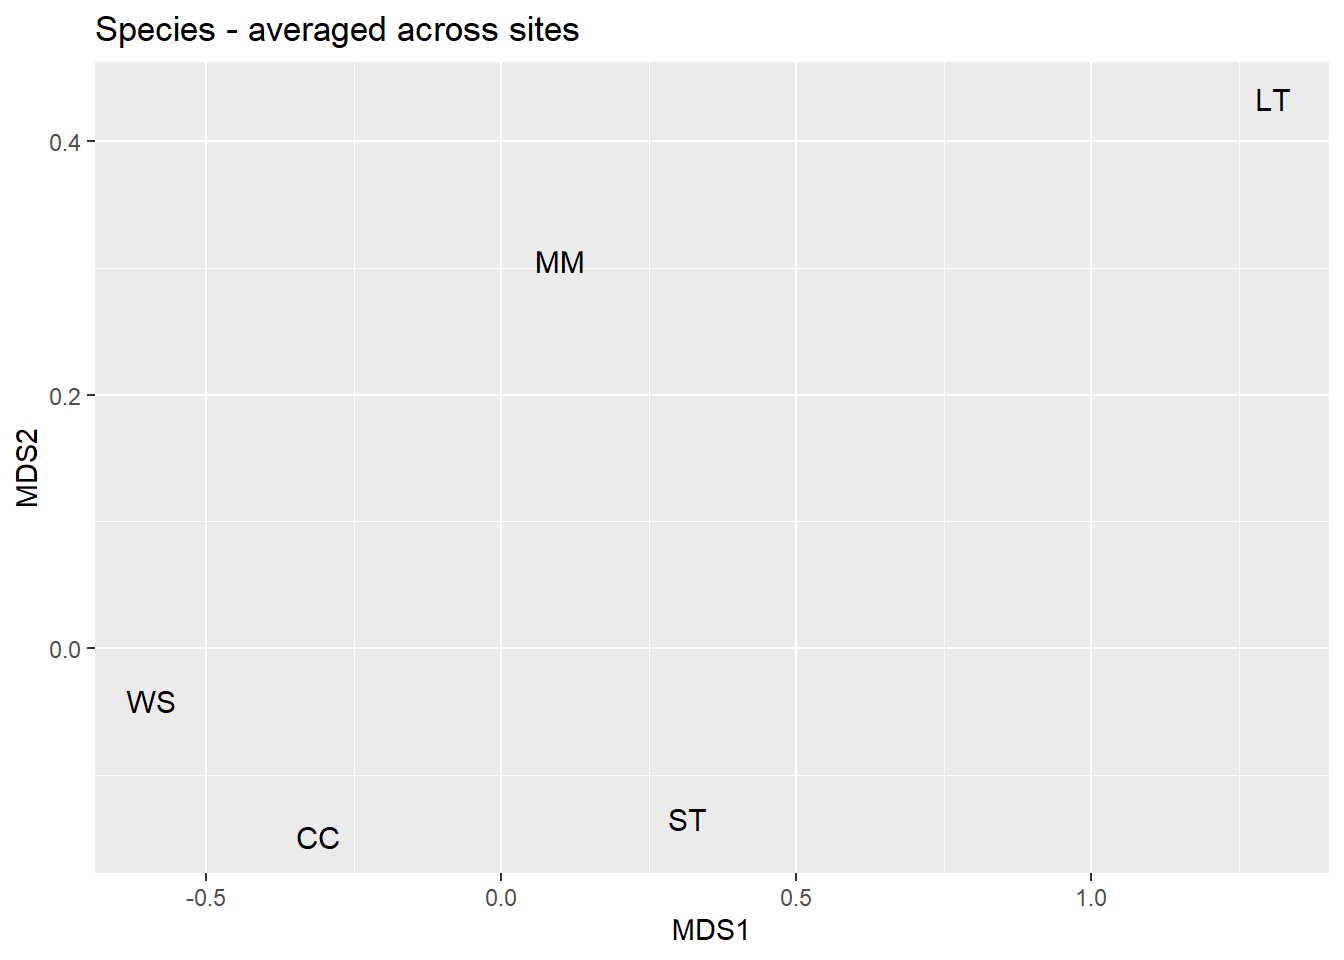
\includegraphics{Chapter_1_files/figure-latex/unnamed-chunk-7-1.pdf}

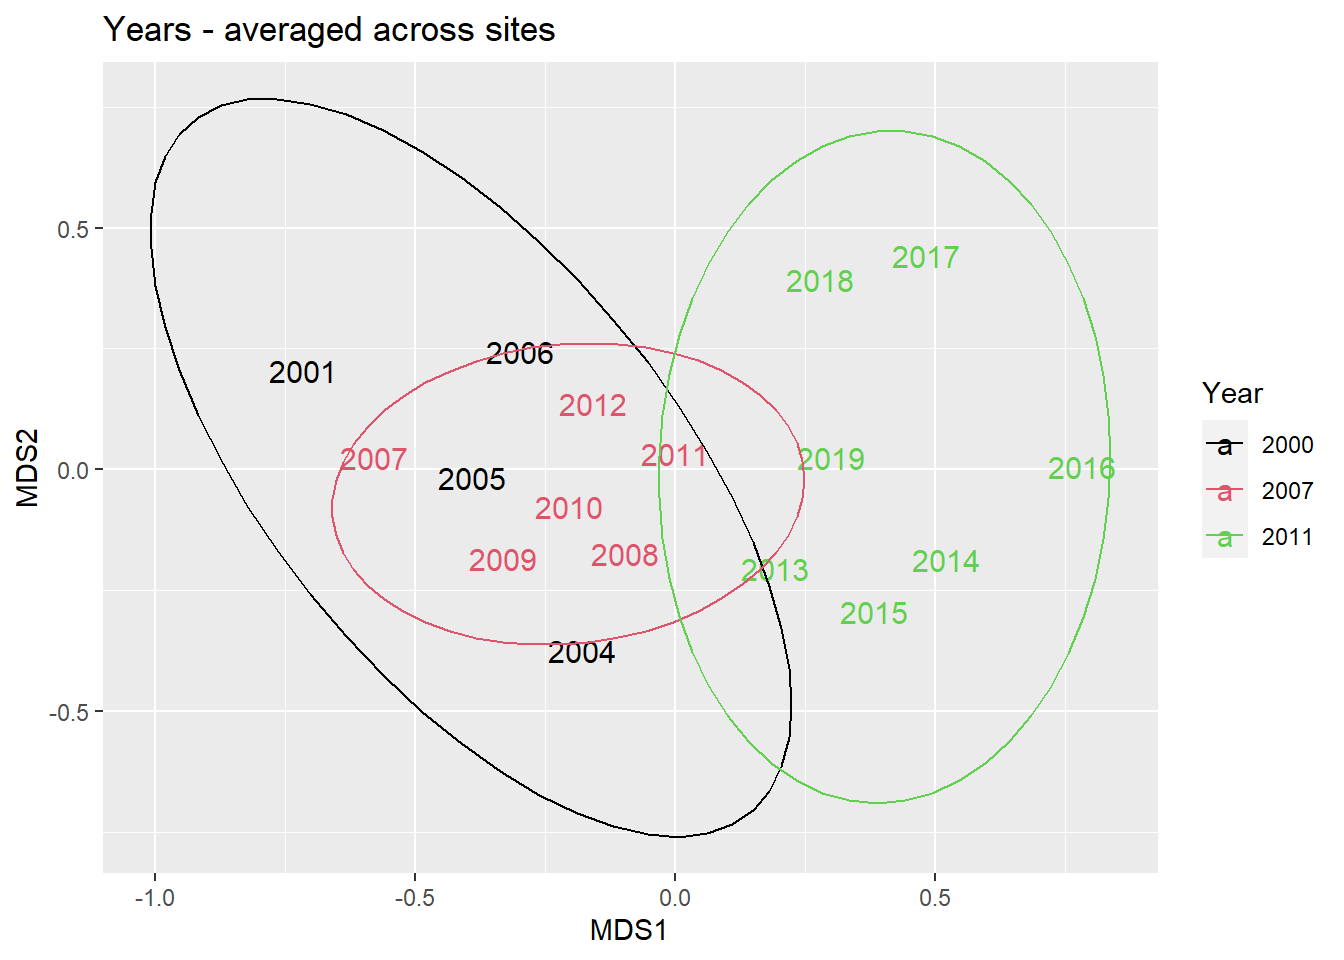
\includegraphics{Chapter_1_files/figure-latex/unnamed-chunk-8-1.pdf}
\#\#\#\# NMDS of ALSC fish communities
----------------------------------------

\begin{verbatim}
## Run 0 stress 0.09413542 
## Run 1 stress 0.09418435 
## ... Procrustes: rmse 0.0008771061  max resid 0.004730678 
## ... Similar to previous best
## Run 2 stress 0.09413884 
## ... Procrustes: rmse 0.0006614536  max resid 0.004565093 
## ... Similar to previous best
## Run 3 stress 0.09415936 
## ... Procrustes: rmse 0.001292873  max resid 0.003951888 
## ... Similar to previous best
## Run 4 stress 0.09414898 
## ... Procrustes: rmse 0.001233892  max resid 0.0050699 
## ... Similar to previous best
## Run 5 stress 0.0941501 
## ... Procrustes: rmse 0.0005891793  max resid 0.00530036 
## ... Similar to previous best
## Run 6 stress 0.09413423 
## ... New best solution
## ... Procrustes: rmse 0.001285819  max resid 0.005726411 
## ... Similar to previous best
## Run 7 stress 0.09415951 
## ... Procrustes: rmse 0.001132009  max resid 0.004749304 
## ... Similar to previous best
## Run 8 stress 0.09418165 
## ... Procrustes: rmse 0.0009591739  max resid 0.004414251 
## ... Similar to previous best
## Run 9 stress 0.09416639 
## ... Procrustes: rmse 0.001395475  max resid 0.005277276 
## ... Similar to previous best
## Run 10 stress 0.09419543 
## ... Procrustes: rmse 0.001037017  max resid 0.003394477 
## ... Similar to previous best
## Run 11 stress 0.09417521 
## ... Procrustes: rmse 0.001021918  max resid 0.004441021 
## ... Similar to previous best
## Run 12 stress 0.09419081 
## ... Procrustes: rmse 0.0008652694  max resid 0.004504415 
## ... Similar to previous best
## Run 13 stress 0.09418762 
## ... Procrustes: rmse 0.0009343011  max resid 0.0046342 
## ... Similar to previous best
## Run 14 stress 0.0941709 
## ... Procrustes: rmse 0.001211126  max resid 0.003632958 
## ... Similar to previous best
## Run 15 stress 0.09417533 
## ... Procrustes: rmse 0.001267874  max resid 0.00467016 
## ... Similar to previous best
## Run 16 stress 0.09413369 
## ... New best solution
## ... Procrustes: rmse 0.00113247  max resid 0.00566548 
## ... Similar to previous best
## Run 17 stress 0.09413538 
## ... Procrustes: rmse 0.001017105  max resid 0.00550883 
## ... Similar to previous best
## Run 18 stress 0.09413278 
## ... New best solution
## ... Procrustes: rmse 0.0005112089  max resid 0.005070399 
## ... Similar to previous best
## Run 19 stress 0.09417409 
## ... Procrustes: rmse 0.001019102  max resid 0.004434459 
## ... Similar to previous best
## Run 20 stress 0.09417872 
## ... Procrustes: rmse 0.0008136175  max resid 0.00423886 
## ... Similar to previous best
## *** Solution reached
\end{verbatim}

\includegraphics{Chapter_1_files/figure-latex/unnamed-chunk-9-1.pdf}

\hypertarget{nestedness-in-alsc-native-fish-communities}{%
\subsection{Nestedness in ALSC Native fish communities
-----------------------------}\label{nestedness-in-alsc-native-fish-communities}}

\begin{verbatim}
## N.columns    N.rows      NODF 
##  76.95728  69.99341  70.68732
\end{verbatim}

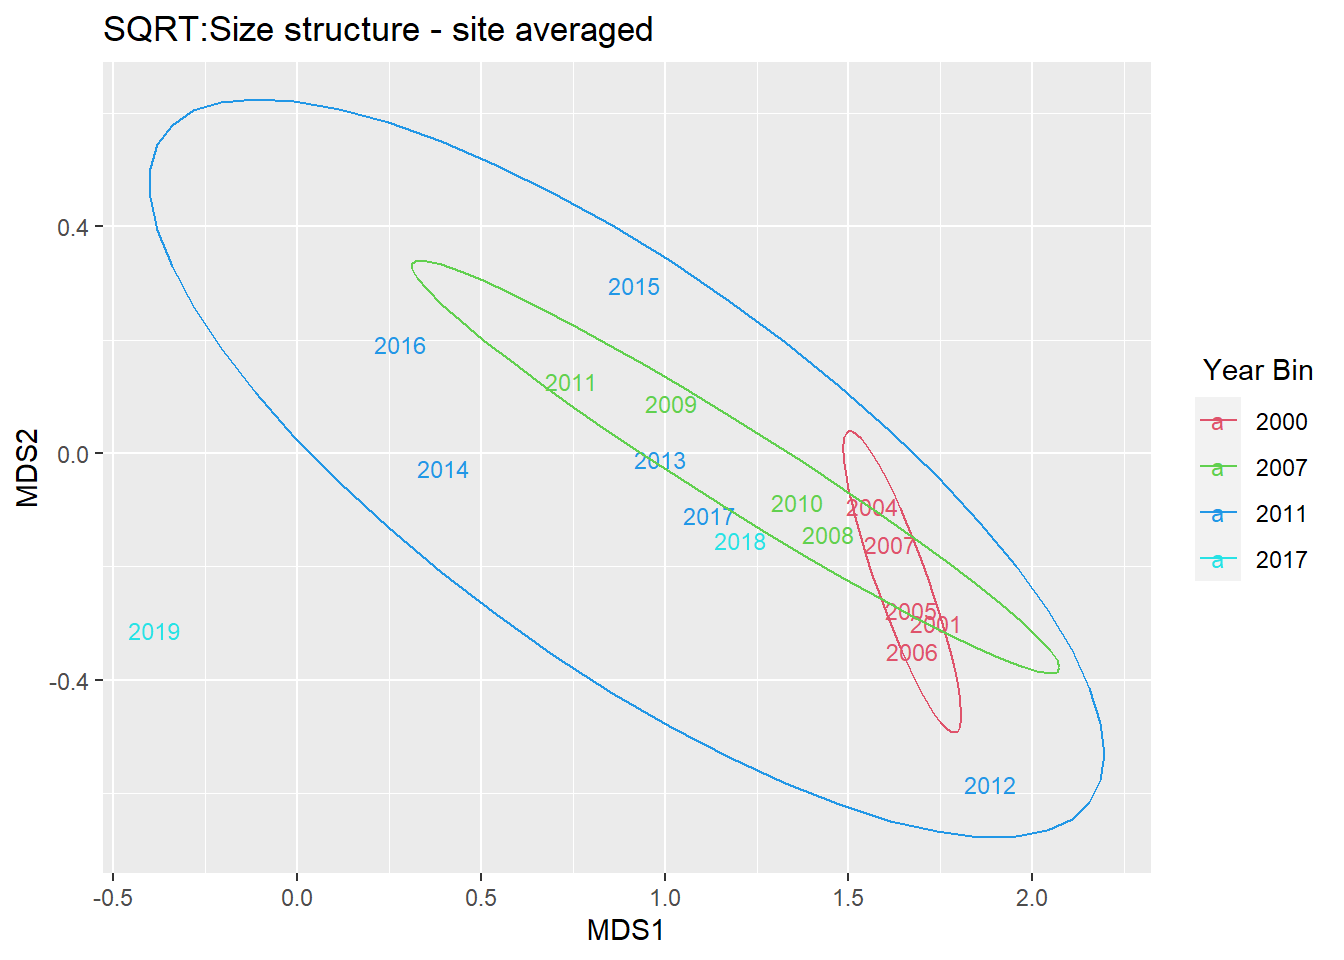
\includegraphics{Chapter_1_files/figure-latex/unnamed-chunk-10-1.pdf}

\hypertarget{trophic-position}{%
\subsection{Trophic position}\label{trophic-position}}

\hypertarget{fishbase}{%
\subsection{Fishbase ---------------------------}\label{fishbase}}

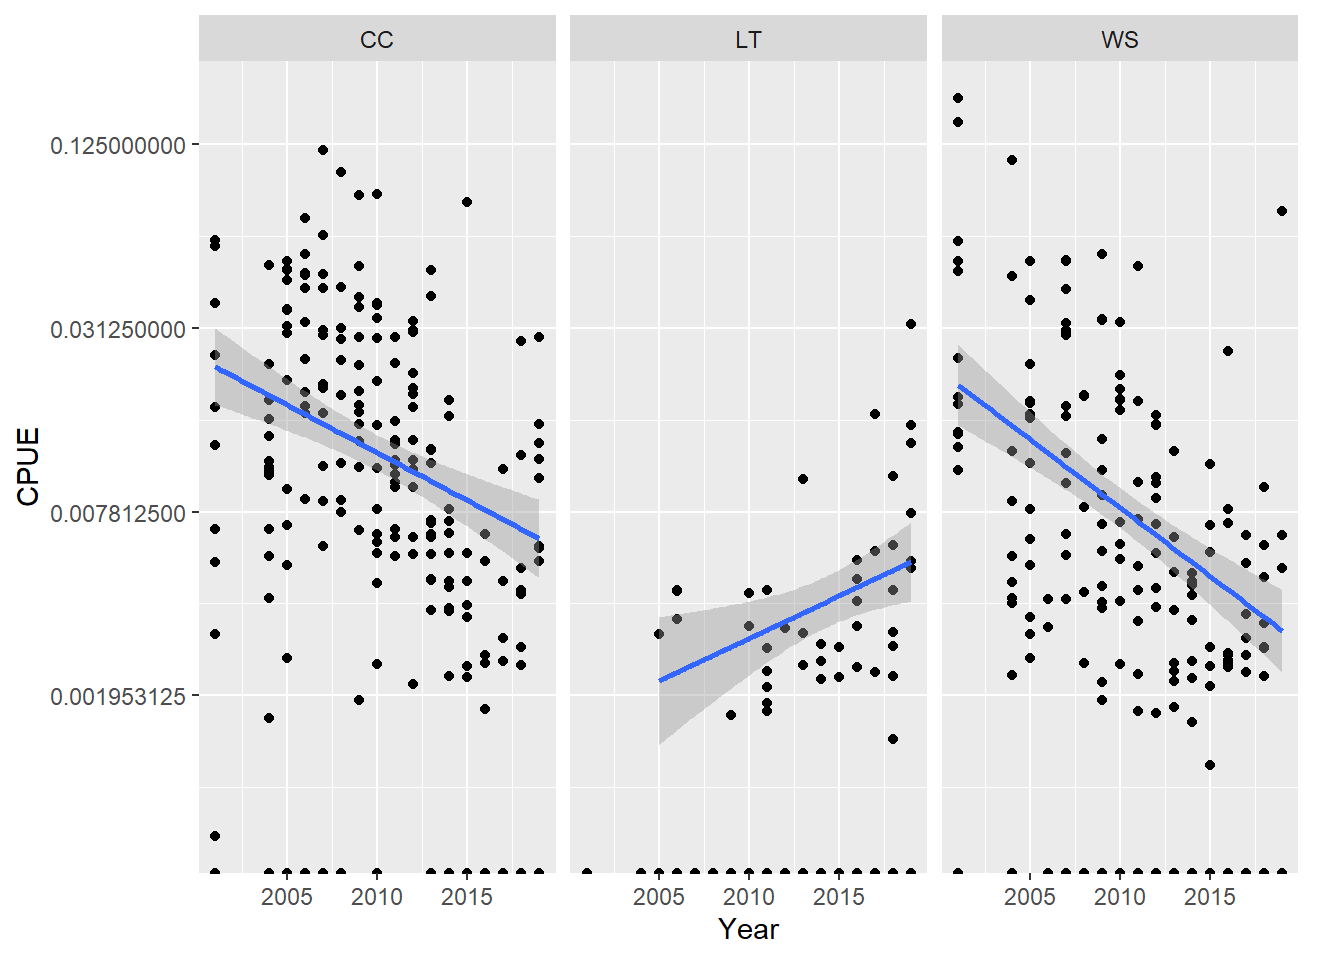
\includegraphics{Chapter_1_files/figure-latex/unnamed-chunk-13-1.pdf}

\hypertarget{predator-presence}{%
\paragraph{Predator Presence
---------------------------------------------------}\label{predator-presence}}

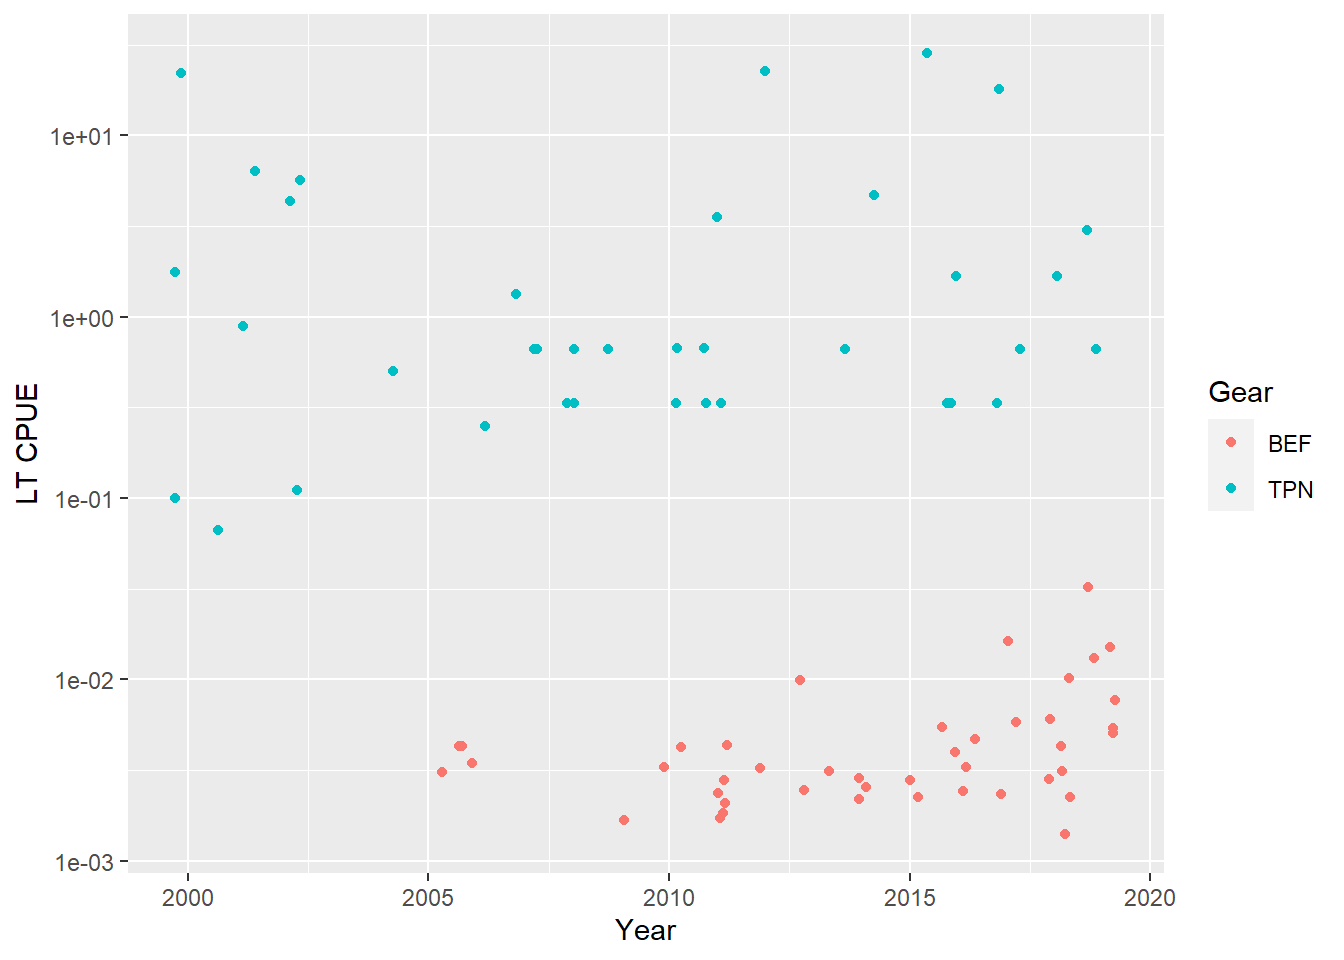
\includegraphics{Chapter_1_files/figure-latex/unnamed-chunk-14-1.pdf}

\end{document}
